% Copyright 2016 - 2017 Bas van Meerten and Wouter Franssen
%
%This file is part of ssNake.
%
%ssNake is free software: you can redistribute it and/or modify
%it under the terms of the GNU General Public License as published by
%the Free Software Foundation, either version 3 of the License, or
%(at your option) any later version.
%
%ssNake is distributed in the hope that it will be useful,
%but WITHOUT ANY WARRANTY; without even the implied warranty of
%MERCHANTABILITY or FITNESS FOR A PARTICULAR PURPOSE.  See the
%GNU General Public License for more details.
%
%You should have received a copy of the GNU General Public License
%along with ssNake. If not, see <http://www.gnu.org/licenses/>.

\documentclass[11pt,a4paper]{article}
% Copyright 2016 - 2017 Bas van Meerten and Wouter Franssen
%
%This file is part of ssNake.
%
%ssNake is free software: you can redistribute it and/or modify
%it under the terms of the GNU General Public License as published by
%the Free Software Foundation, either version 3 of the License, or
%(at your option) any later version.
%
%ssNake is distributed in the hope that it will be useful,
%but WITHOUT ANY WARRANTY; without even the implied warranty of
%MERCHANTABILITY or FITNESS FOR A PARTICULAR PURPOSE.  See the
%GNU General Public License for more details.
%
%You should have received a copy of the GNU General Public License
%along with ssNake. If not, see <http://www.gnu.org/licenses/>.

\usepackage[british]{babel}
\usepackage{graphicx,booktabs,listings,amsmath,pgfplots,pgfplotstable}
\usepackage[small,bf,nooneline]{caption}
\usepackage{subcaption}
\usepackage[sort&compress,numbers]{natbib}
\usepackage{tikz}
\usepackage{mathtools}
\usepackage[nottoc]{tocbibind}%adds bibliography to table of contents.
\graphicspath{{./images/}}
%\setlength{\textwidth}{453pt} %597 pt is the a4 paperwidth. Minus 2 in margin. 72 pt = 1 in
%\setlength{\hoffset}{-\oddsidemargin}
%\setlength{\voffset}{-30pt} %
%\setlength{\textheight}{651 pt} %a4 height 845 pt minus 2* total headheight. In this case 2*88pt
%% examine margines via the layout package. Use command \layout{} in document to draw a picture.
%\setlength{\parindent}{0.5 cm}
%\setlength{\parskip}{0 cm}
\usepackage[left=82pt,right=82pt,top=95pt,bottom=95pt,footnotesep=0.5cm]{geometry}
%\setlength{\headheight}{14pt}

%define colours--------------------
%dark
\usepackage{xcolor}
\definecolor{MyGrayD}{RGB}{1,1,1}
\definecolor{MyRedD}{RGB}{237,45,46}
\definecolor{MyGreenD}{RGB}{0,140,71}
\definecolor{MyBlueD}{RGB}{24,89,169}
\definecolor{MyOrangeD}{RGB}{243,125,34}
\definecolor{MyPurpleD}{RGB}{102,44,145}
\definecolor{MyBrownD}{RGB}{161,29,32}
\definecolor{MyPinkD}{RGB}{179,56,147}
%normal
\definecolor{MyGray}{RGB}{114,114,114}
\definecolor{MyRed}{RGB}{241,89,95}
\definecolor{MyGreen}{RGB}{121,195,106}
\definecolor{MyBlue}{RGB}{89,154,211}
\definecolor{MyOrange}{RGB}{249,166,90}
\definecolor{MyPurple}{RGB}{158,102,171}
\definecolor{MyBrown}{RGB}{205,112,88}
\definecolor{MyPink}{RGB}{215,127,179}
%light
\definecolor{MyGrayL}{RGB}{204,204,204}
\definecolor{MyRedL}{RGB}{242,174,172}
\definecolor{MyGreenL}{RGB}{216,228,170}
\definecolor{MyBlueL}{RGB}{184,210,235}
\definecolor{MyOrangeL}{RGB}{242,209,176}
\definecolor{MyPurpleL}{RGB}{212,178,211}
\definecolor{MyBrownL}{RGB}{221,184,169}
\definecolor{MyPinkL}{RGB}{235,191,217}
%----------------------------------

%Figure ref with hyperref
\newcommand{\fref}[1]{\hyperref[#1]{Figure \ref*{#1}}}
\newcommand{\sref}[1]{\hyperref[#1]{Section \ref*{#1}}}
\newcommand{\tref}[1]{\hyperref[#1]{Table \ref*{#1}}}

%Makes a new command for figures with input values: filename, width(times linewidth),
% caption and label.
\newcommand{\onefigure}[4]{
\setlength{\captionwidth}{#2\linewidth}
\begin{figure}
\includegraphics[width=#2\linewidth]{#1}
\centering
\parbox{\linewidth}{\caption{#3}
\label{#4}}
\end{figure}
}

%Makes a new command for tikz figures with input values: tikz commands, 
% caption and label.
\newcommand{\onetikz}[3]{
\settowidth{\captionwidth}{#1}
\ifthenelse{\lengthtest{\captionwidth<0.7\linewidth}}{\setlength{\captionwidth}{0.7\linewidth}}{}

\begin{figure}
\centering
#1
\centering
\parbox{\linewidth}{\caption{#2}
\label{#3}}
\end{figure}
}

%Makes a new command for two figures next to each other with input values: filename1, caption1, label1,filename2, caption2 and label2. Figure width is set to 0.47\linewidth and the space between the figures is filled with \hfill so the sides of the figures align with to edge of the line.
\newcommand{\twofigure}[6]{
\setlength{\captionwidth}{\linewidth}
\begin{figure*}[ht!]
\begin{minipage}[t]{0.47\linewidth}
\includegraphics[width=\linewidth]{#1}
\centering
\caption{#2}
\label{#3}
\end{minipage}
\hfill
\begin{minipage}[t]{0.47\linewidth}
\centering
\includegraphics[width= \linewidth]{#4}
\centering
\caption{#5}
\label{#6}
\end{minipage}
\end{figure*}
}


%Makes a new command for a table with caption witdh equal to the total table width. Input: tabular, caption and label. Example:
%\onetable{
%\begin{tabular}{ccc}
%a&b&c\\
%\hline
%1&1&1\\
%1&1&1\\
%1&1&1\\
%\end{tabular}
%{The caption.}
%{tab:table1}
%}
\newcommand{\onetable}[3]{
\settowidth{\captionwidth}{#1}
\ifthenelse{\lengthtest{\captionwidth<0.7\linewidth}}{\setlength{\captionwidth}{0.7\linewidth}}{}
\begin{table}
\caption{#2}
\vspace{-0.24cm} %Puts caption close to toprule
\label{#3}
\centering
#1
\end{table}
}

%Makes a long table with captionwidth equal to tablewidth. It takes the following arguments:
%1: Column specifier (e.g. cccc)
%2: Caption
%3: Label
%4: First head (i.e. first row of regular table)
%5: Head of consecutive pages
%6: Foot of pagebreak
%7: Lastfoot (e.g. \midrule)
%8: Body of table
\newcommand{\onelongtable}[8]{
\begin{center}
\settowidth{\captionwidth}{
\begin{tabular}{#1}
#4
#8
\end{tabular}} % This ends the captionwidth part. Next comes the real table.

\begin{longtable}{#1}
\caption{#2}\\
\vspace{-0.74cm} %Puts caption close to toprule
\label{#3}\\

#4
\endfirsthead

#5
\endhead

#6
\endfoot

#7
\endlastfoot

#8
\end{longtable}
\end{center}}




%1:pgfplots code
%2:width
%3:caption
%4:label
\newcommand{\pgfplotsfigure}[4]{
\pgfplotsset{width=#2\linewidth}
\setlength{\captionwidth}{#2\linewidth}
\begin{figure}[t]
\centering
#1
\centering
\parbox{\linewidth}{\caption{#3}
\label{#4}}
\end{figure}
}


\usepackage[bitstream-charter]{mathdesign}
\usepackage[T1]{fontenc}
\usepackage[protrusion=true,expansion,tracking=true]{microtype}
\pgfplotsset{compat=1.7,/pgf/number format/1000 sep={}, axis lines*=left,axis line style={gray},every outer x axis line/.append style={-stealth'},every outer y axis line/.append style={-stealth'},tick label style={font=\small},label style={font=\small},legend style={font=\footnotesize}}
\usepackage{colortbl}
\usetikzlibrary{calc}

%Set section font
\usepackage{sectsty}
\allsectionsfont{\color{black!70}\fontfamily{SourceSansPro-LF}\selectfont}
%--------------------


%Set toc fonts
\usepackage{tocloft}
%\renewcommand\cftchapfont{\fontfamily{SourceSansPro-LF}\bfseries}
\renewcommand\cfttoctitlefont{\color{black!70}\Huge\fontfamily{SourceSansPro-LF}\bfseries}
\renewcommand\cftsecfont{\fontfamily{SourceSansPro-LF}\selectfont}
%\renewcommand\cftchappagefont{\fontfamily{SourceSansPro-LF}\bfseries}
\renewcommand\cftsecpagefont{\fontfamily{SourceSansPro-LF}\selectfont}
\renewcommand\cftsubsecfont{\fontfamily{SourceSansPro-LF}\selectfont}
\renewcommand\cftsubsecpagefont{\fontfamily{SourceSansPro-LF}\selectfont}
%--------------------

%Define header/foot
%\usepackage{fancyhdr}
%\pagestyle{fancy}
%\fancyhead[LE,RO]{\fontfamily{SourceSansPro-LF}\selectfont \thepage}
%\fancyhead[LO,RE]{\fontfamily{SourceSansPro-LF}\selectfont \leftmark}
%\fancyfoot[C]{}
%--------------------

%remove page number from first chapter page
%\makeatletter
%\let\ps@plain\ps@empty
%\makeatother
%----------------------

\usepackage[hidelinks,colorlinks,allcolors=black, pdftitle={QCPMG},pdfauthor={Wouter M.J.\ Franssen}]{hyperref}

\interfootnotelinepenalty=10000 %prevents splitting of footnote over multiple pages
\linespread{1.2}

\title{\color{black}\fontfamily{SourceSansPro-LF}\bfseries QCPMG processing in ssNake}
\author{}
\date{\color{black}\fontfamily{SourceSansPro-LF}\bfseries \today}


\begin{document}
%\newgeometry{left=72pt,right=72pt,top=95pt,bottom=95pt,footnotesep=0.5cm}
\microtypesetup{protrusion=true} % enables protrusion

\maketitle

\section{Introduction}
The following will explain how QCPMG NMR data can be processed in ssNake.
 The
tutorial delivered with the ssNake program is considered as prior knowledge. If you have not yet
studied this, please do so before continuing with this example.

QCPMG-sequence stands for Quadrupolar Carr-Purcell-Meiboom-Gill sequence. The sequence is used to
measure a consecutive series of echoes, which are all recorded. Via careful processing the
signal-to-noise ratio of this data can be higher that if only a single echo would have been
recorded. The experiment is particularly helpful for broad quadrupolar patterns, where the decay of
the signal is much faster than the intrinsic decay of the magnetization ($T_2$). In this case, many
echoes can be recorded in one go.

QCPMG experiments can be processed in number of ways to produce either a spikelet pattern, or a more
regular NMR spectrum. Both have their advantages in specific circumstances.


\section{Data}
The used data is a $^{35}$Cl spectrum of magnesium chloride (MgCl$_2$) recorded at 20 T using 15.6
kHz MAS.


\section{Processing}
\subsection{Sum echo spectrum}
The most general way of analysing the series of echoes that are recorded in a QCPMG experiment is by
adding all the individual echoes, and process it as you would a single echo experiment. This
gives a spectrum that is easy to interpret and has a higher signal-to-noise when compared to a
regular echo. However, processing can be tricky, and requires a careful method.

The data supplied in this tutorial has 137 measured echoes, consisting of 1088 data points each. In
order to add these, we must split the data in 137 parts, to form a pseudo 2D data set with shape
$137 \times 1088$. Setting the number of echoes is done when measuring the spectrum, but can also
be counted afterwards. Getting the number of points can be more tricky. Dividing the number of data
points by 137 should give this, but in our case the QCPMG data has zeroes appended to the echoes.
What we do know is that only with the correct number of points (1088) the splitting of the data
gives an aligned result.

\begin{itemize}
  \item Open the data in the \texttt{Raw} directory
\end{itemize}
Each echo has some zeroes appended to it, which is a consequence of how the Varian equipment is
measuring the QCPMG data. This can be seen in the following Figure (from the start of the FID):
\begin{center}
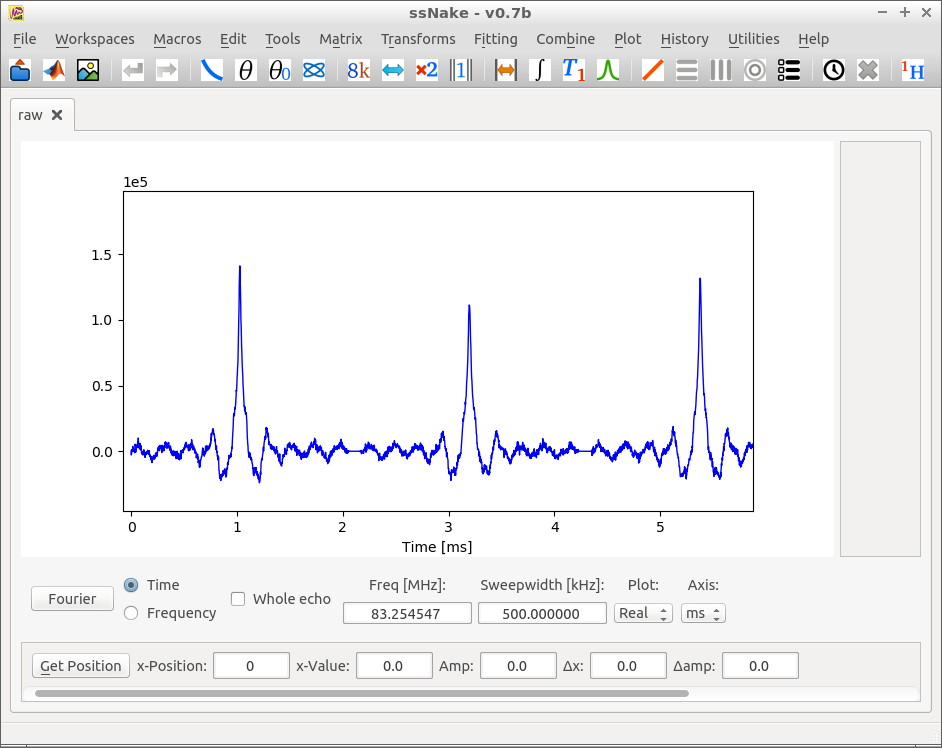
\includegraphics[width=0.7\linewidth]{Figs/Fig1.png}
\end{center}
which shows the first 2 and a half echoes. We now must split the data in the 137 echoes.
\begin{itemize}
  \item Set the size to $137 \cdot 1088 = 149056$ data points (Matrix $\longrightarrow$ Sizing)
  \item Split the data: Matrix $\longrightarrow$ Split (137 sections)
\end{itemize}
Now we have all the separate echoes. Viewing D2 gives:
\begin{center}
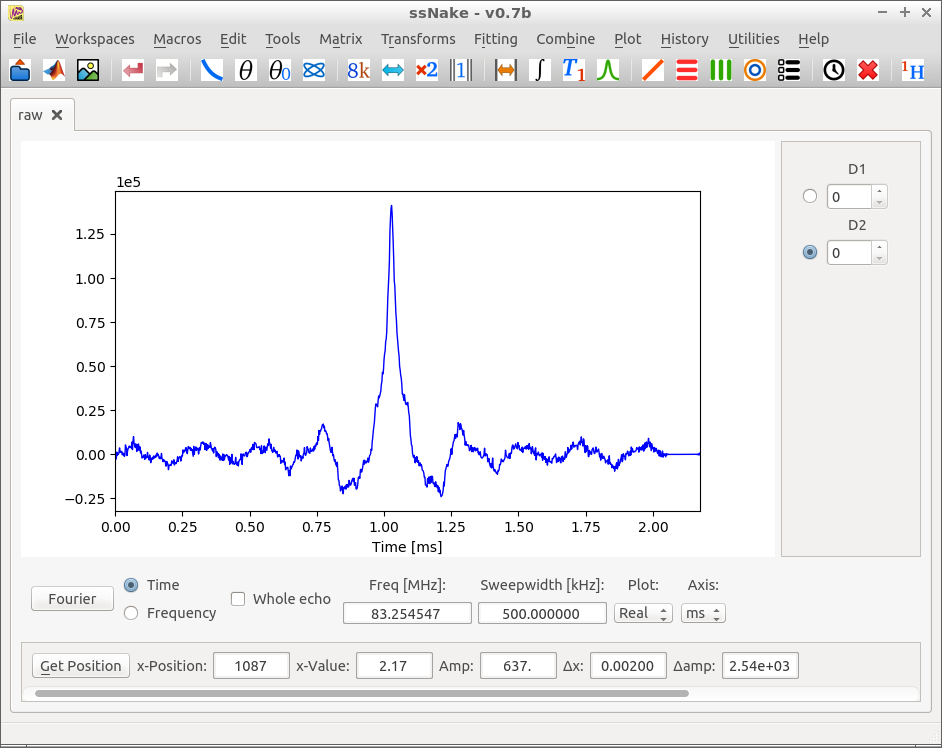
\includegraphics[width=0.7\linewidth]{Figs/Fig2.png}
\end{center}
which shows the first echo. Scrolling through D1, we can see that for each echo, the position is the
same: the splitting has been performed correctly. A stack plot of the first 10 echoes for example
gives:
\begin{center}
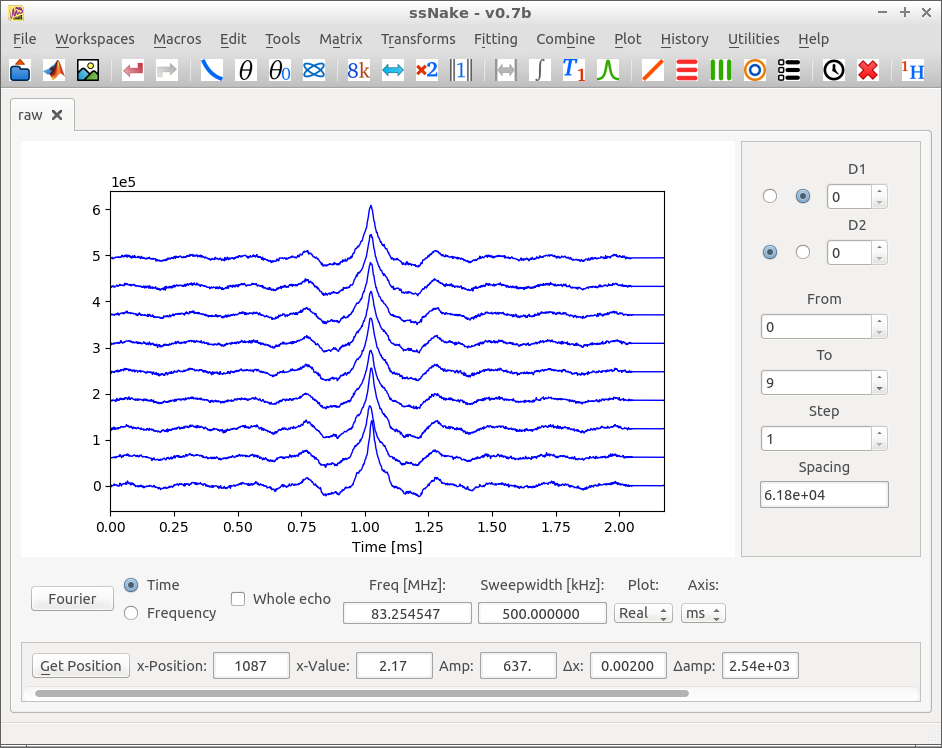
\includegraphics[width=0.7\linewidth]{Figs/Fig3.png}
\end{center}
which looks good. If we had used 1000 points per echo we would see:
\begin{center}
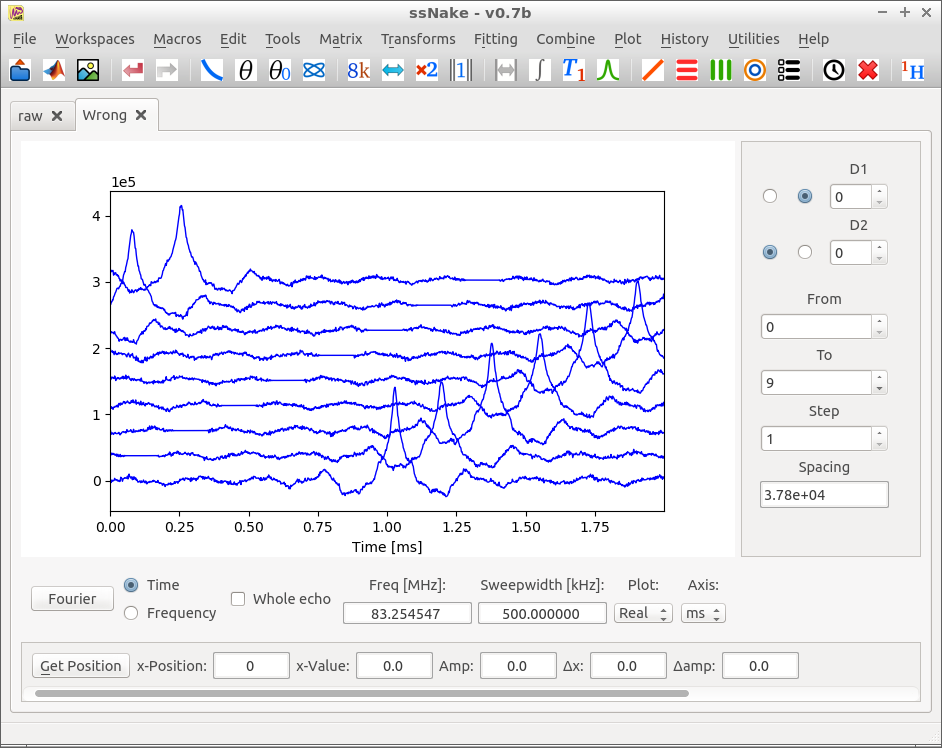
\includegraphics[width=0.7\linewidth]{Figs/Fig4.png}
\end{center}
which is clearly very, very, wrong. A good check is to overlay the first and last echo. The `zero'
part at the end should be at the same position.

\subsubsection{Option 1: Directly summing the echoes}
Using the properly split data we can sum the echoes:
\begin{itemize}
  \item Go to D1 (using the radio button in the side frame)
  \item Sum along this dimension using: Matrix $\longrightarrow$ Region $\longrightarrow$ Sum (with
	 no input, just push Ok).
\end{itemize}
This gives:
\begin{center}
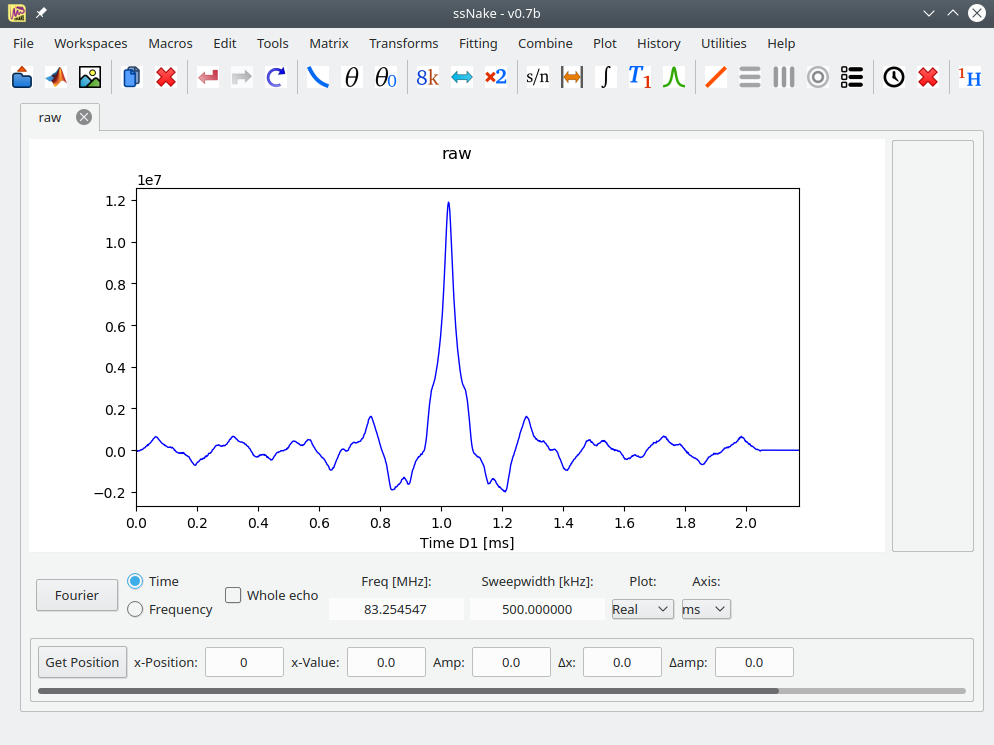
\includegraphics[width=0.7\linewidth]{Figs/Fig5.png}
\end{center}

We will now process the data using whole echo processing. More on this can be found in the Whole
Echo processing tutorial. In short:
\begin{itemize}
  \item Swap the echo using Tools $\longrightarrow$ Swap echo at point 512
  \item Zero fill to 8192 points using Matrix $\longrightarrow$ Sizing
  \item Fourier transform with the Fourier button in the bottom frame
  \item Phase a bit using Tools $\longrightarrow$ Phasing (0th order: 0.220, 1st order: 68)
  \item 800 Hz Gaussian apodization (Tools $\longrightarrow$ Apodize)
\end{itemize}
This shows (zoomed):
\begin{center}
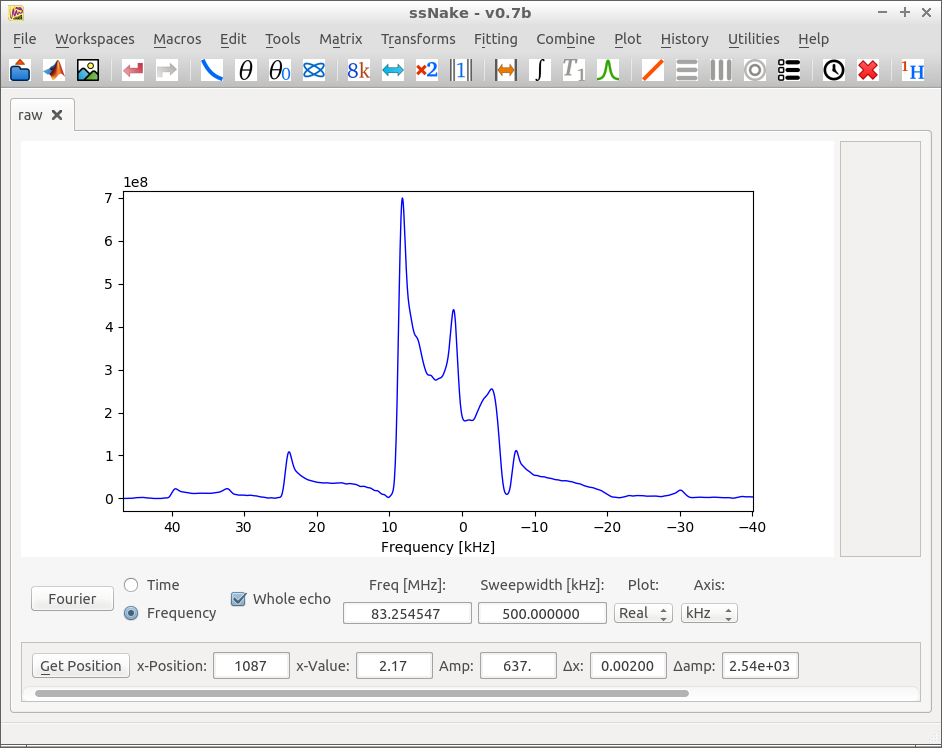
\includegraphics[width=0.7\linewidth]{Figs/Fig6.png}
\end{center}
Which is the final spectrum using this processing method. It is saved as \texttt{EchoSumOption2.mat}
in the data directory.

\subsubsection{Option 2: T2 weighting}
Summing all the echoes as has been done in Option 1 is fine in some cases, but can lead to signal-to-noise
drawbacks. We are adding the echoes to gain a higher signal-to-noise when compared to a single echo
experiment (and not a QCPMG). But what if our last echo has no signal anymore? Clearly, adding this
echo only introduces noise into our sum of echoes. We want only to add echoes that give us a gain in
signal-to-noise. The best way to do this seems to multiply all our 137 echoes by their maximum
intensity: weak echoes with only noise have hardly any intensity, and are reduced, while intense
echoes get a good boost. As the echo intensity is reducing due to $T_2$ effects, this scaling method
is often called `$T_2$ weighting'.

To perform a $T_2$  weighting, we must first get the $T_2$. We start with the data on which we have
just done the splitting in 137 parts (before the Option 1 section processing). The echo tops are in
this case located at data point 514. Fill in this number in the D2 box and press enter. This should
give:
\begin{center}
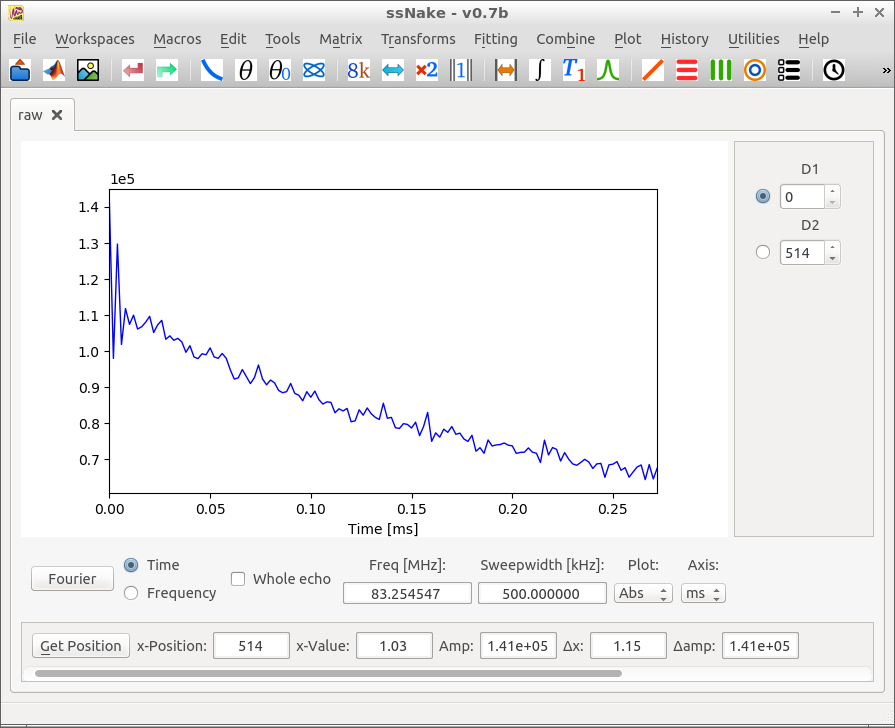
\includegraphics[width=0.7\linewidth]{Figs/Fig7.png}
\end{center}

We now want to fit this line with a $T_2$ decay. DO note that the spectral width in this case was
invented by ssNake. This means that our fitted $T_2$ will be in a random unit, but as long as we
apply the weighting in the same unit, we should be fine\footnote{Alternatively, we could define the
spectral width as the inverse of the time between the echo tops.}. Let's fit a $T2$:

\begin{itemize}
  \item Open the relaxation fitting frame (Fitting $\longrightarrow$ Relaxation Curve)
	\item Set the `Constant' at 0, and the `Coefficient' at 1
	\item Set the `T' variable at 0.001 as an initial guess
	 \item Tick the boxes next to the `Constant' and `Coefficient' (this makes them fixed, so that they
		do not change during the fitting)
	\item Push `Fit' (and a second time to get a better result)
\end{itemize}
This gives:
\begin{center}
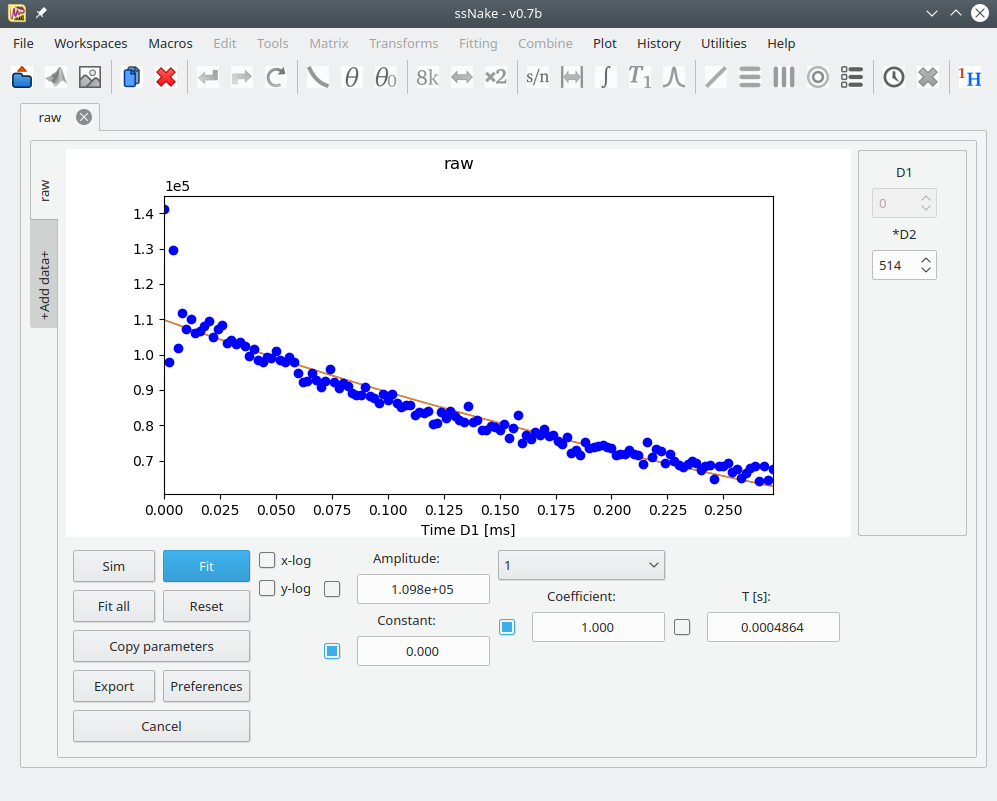
\includegraphics[width=0.7\linewidth]{Figs/Fig8.png}
\end{center}
with a $T_2$ of 0.0004865 second. Close the Window using the `Cancel' button

We now wish to use this $T_2$ to scale our echo intensities. We will do this using Lorentzian
apodization, which has the same function as a $T_2$ decay (exponential decay). The value that we
will use is: $\text{LB} = 1/(T_2 \cdot \pi) = 654$ Hz.


\begin{itemize}
  \item Use Tools $\longrightarrow$ Apodize and apply 654 Hz Lorentzian apodization along D1
\end{itemize}
The data can now be further processed using the methods of Option 1 above. This $T_2$ weighted
spectrum should have a better signal-to-noise that that of Option 1, although this particular data
has no really low intensity echoes, so the difference will be small. The final spectrum is saved in
the data directory as \texttt{EchoSumOption2.mat}.





\subsection{Spikelet spectrum}
A wholly different method for processing the data from a QCPMG experiment is the spikelet method. It
features a direct Fourier transform of the FID, with no splitting and summing of the echoes. The
spectrum it leads to has a series of spikes (i.e. spikelets) in the spectrum, with a distance of $1 /T$
, with $T$ the time between two echoes. The advantage of the spikelet method is that all the
signal is concentrated in the spikes, leading to a huge increase in signal-to-noise ratio. The disadvantage is
that, while the tops of the spikes follow the intensity distribution of the `regular' echo spectrum,
the area betwene the spikes gives no information. If only a few spikelets are present, the shape of
the quadrupolar line becomes obscured. 


\begin{itemize}
  \item Open the data in the \texttt{Raw} folder
	\item Zero fill to 524288 (Matrix $\longrightarrow$ Sizing)
\end{itemize}
We now need to apply a first order phase correction, to make sure the FID starts at the first echo
top. The position of this top is data point 514. To correct this we need $\theta = 360 \cdot n =
185040$ degrees first order phasing:


\begin{itemize}
  \item Phase with 185040 first order phasing (Tools $\longrightarrow$ Phasing)

\end{itemize}
And to get a good spectrum:
\begin{itemize}
	\item Fourier transform (using the `Fourier' button)
	\item Gaussian apodization of 4 Hz
	\item Phase (0th order: -104, 1st order: -618)
\end{itemize}
This gives the final spectrum: 
\begin{center}
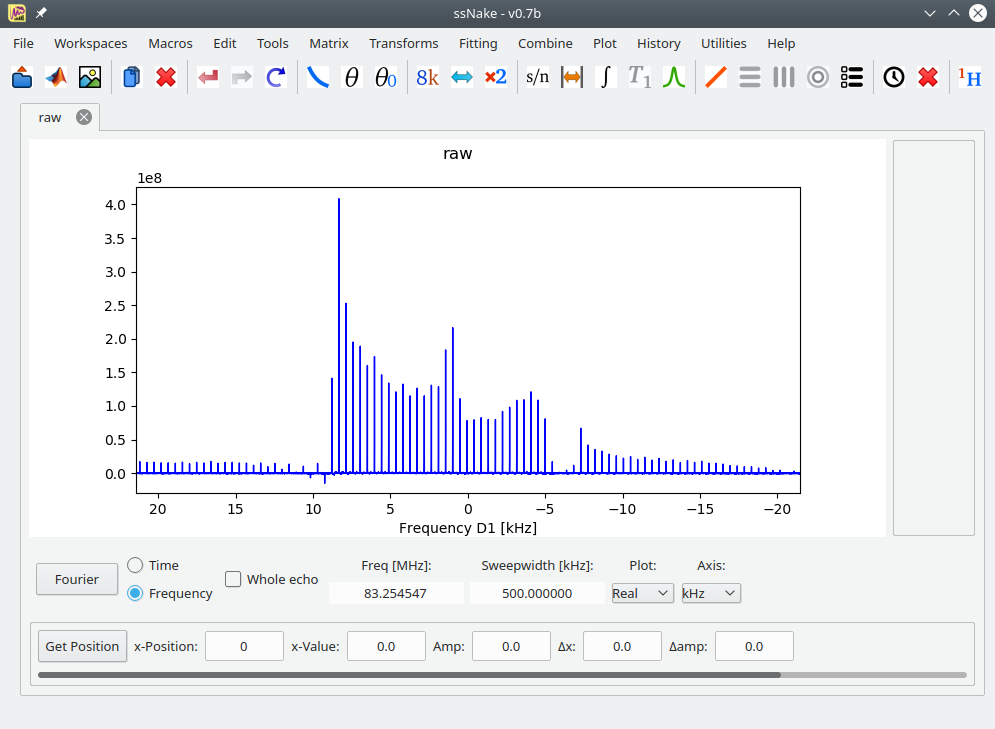
\includegraphics[width=0.7\linewidth]{Figs/Fig9.png}
\end{center}
which is saved as \texttt{spikelets.mat} in the data folder.

When we performed the Gaussian apodization, we also removed the tail of the first echo (which was
shifted to the end of the FID by the large first order phase correction). This suppresses the
formation of a regular echo line shape under our QCPMG spikelets at the cost of intensity. In this
case, we have many intense echoes, and the added baseline of this tail does not help us. If we do
wish to retain this, we must make sure that the apodization is performed \textit{before} the large
first order phase shift.





\end{document}
